\subsection{Energy Manifold}
The energy manifolds intention is be a diversion module to as many different subunits as needed for fluid diversion. It consists of a series of pipes that can be extended to “n” submodules, see Figure \ref{Top View Energy Manifold}. The unit has the capability of utilizing control schemes, however in many practical applications the control schemes are encapsulated within the subprocesses as opposed to within the energy manifold. There are currently four potential energy manifolds that can be used. For practical purposes only the model SteamManifold\textunderscore L1\textunderscore boundaries is used in integrated energy systems as it does not include control valves and supports “n” submodules going in and out. The other versions of the energy manifold exist for advanced users in the event the balance of plant or subprocess they are connecting to does not include sufficient valving and control to properly constrain the system. For example, simplified balance of plant systems that do not contain return flow would require the energy manifold to provide makeup water from the condenser, therefore for that scenario we would need to use the SteamManifold\textunderscore L1\textunderscore FWH\textunderscore Cond model which contains a condenser and feedwater heater.   

\begin{figure}[hbtp]
\centering
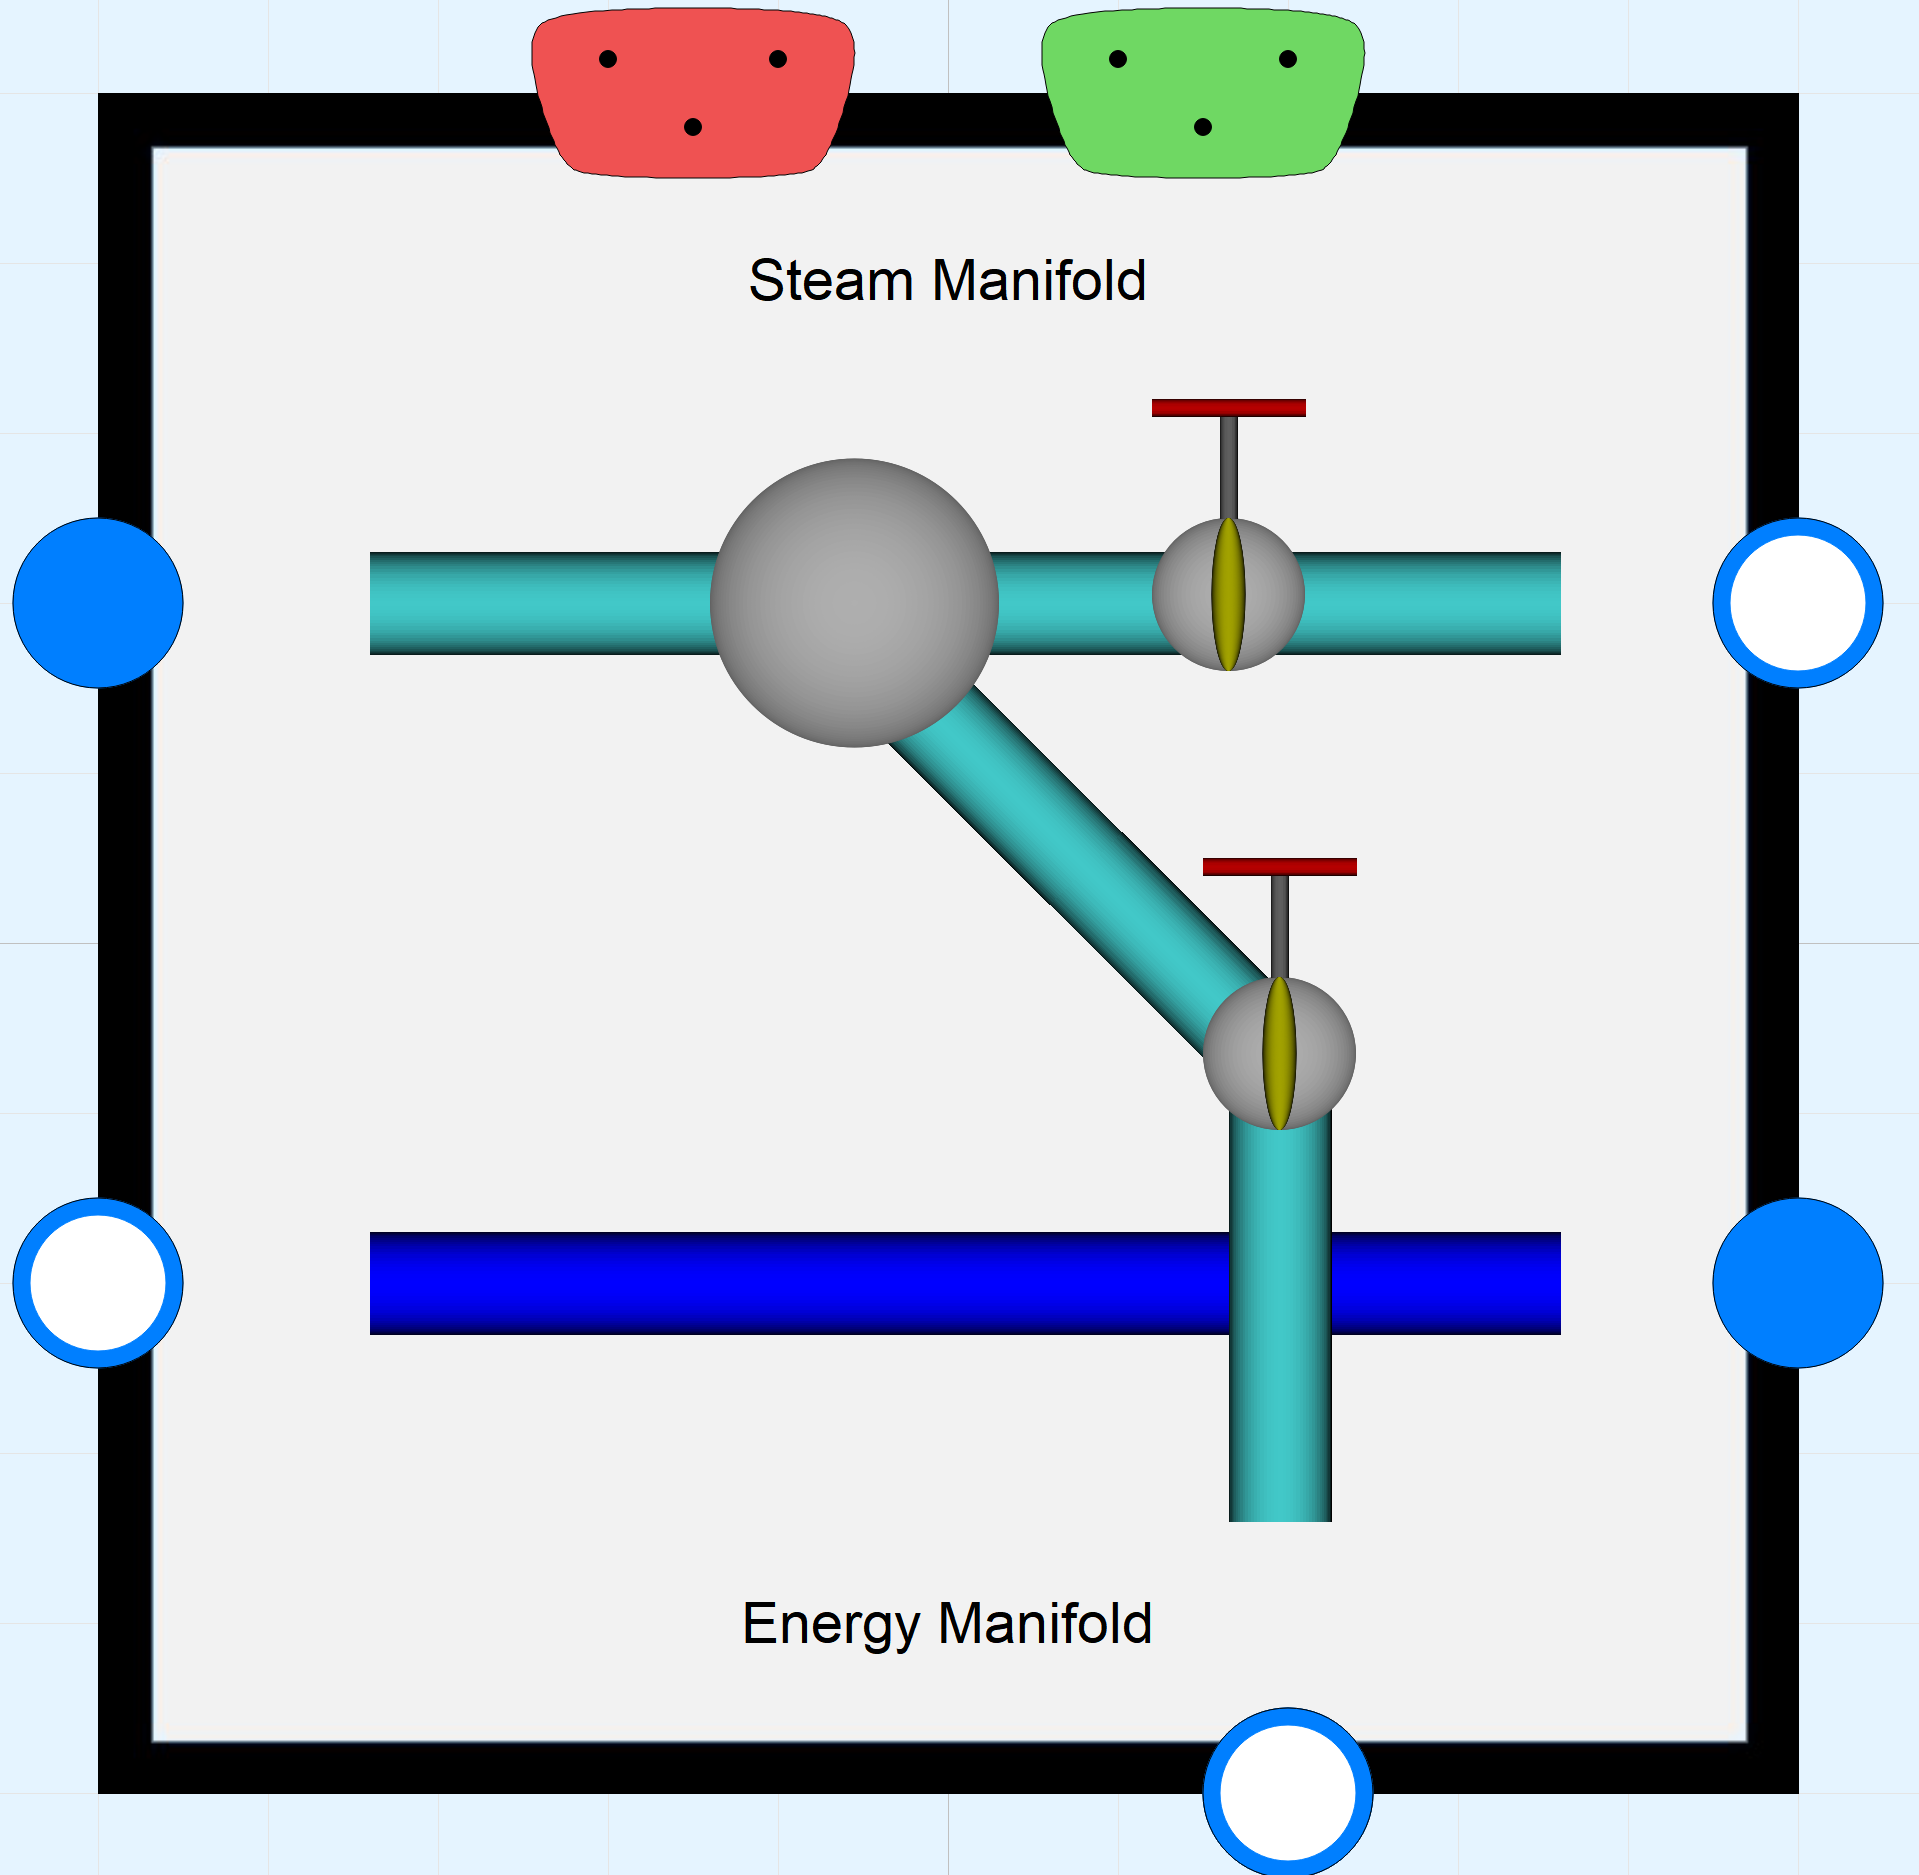
\includegraphics[scale=0.15]{pics/Energy_Manifold.png}
\caption{: Top Level Depiction of the Energy Manifold in the NHES package}
\label{Top View Energy Manifold}
\end{figure}



% content


%\subsection{Cloning the Hybrid Repository}
\label{sec:clone raven}

The first step in installing the package is to clone the HYBRID repository. To do this, use
\begin{lstlisting}[language=bash]
git clone git@hpcgitlab.inl.gov:hybrid/hybrid.git
\end{lstlisting}
This will download the repository into a folder called 'hybrid'. To go inside the folder, use
\begin{lstlisting}[language=bash]
cd hybrid
\end{lstlisting}

\begin{list}{}{}
\item Note: This only works if you have access to the HYBRID repository.

\item Note2: If you are outside INL, be sure you have the ssh tunnel to INL set-up. For instructions, please check the \href{http://mooseframework.org/wiki/hpcgitlabconnectivity/}{HPC GitLab Connectivity} page.

\item Note3: Be sure to have the proxy settings correct. See \href{https://github.com/idaholab/raven/wiki}{RAVEN} wiki .

\item Note4: An ssh key needs to be registered for hpcgitlab.inl.gov. This key should be good for both, the HYBRID repository as well as the CashFlow plugin. Instructions to generate and register ssh keys can be found \href{https://hpcgitlab.inl.gov/help/ssh/README}{here}.
If you have troubles accessing the repository, see \href{/hybrid/hybrid/wikis/Install_troubles}{Installation trouble shooting}.
\end{list}

\subsubsection{Install RAVEN and its plugins as a sub-module}

The next step is to download and install RAVEN and the submodule (e.g. TEAL, HERON) plugins as a sub-module of the HYBRID repository. 

A submodule allows you to keep another Git repository in a subdirectory of your repository. The other repository has its own history, which does not interfere with the history of the current repository. This can be used to have external dependencies such as third party libraries for example.

In order to get RAVEN do the following in the hybrid folder

\begin{lstlisting}[language=bash]
git checkout devel
\end{lstlisting}

Update the Branch

\begin{lstlisting}[language=bash]
git pull
\end{lstlisting}

to add RAVEN as a submodule
\begin{lstlisting}[language=bash]
git submodule update --init --recursive
\end{lstlisting}

\textbf{Install and Compile RAVEN. }
Once you have downloaded RAVEN as a sub-module, you have to install it. go to the \href{https://github.com/idaholab/raven/wiki/intallationMain}{RAVEN Wiki} for information about how to install it. Run all the tests outlined in the RAVEN wiki. 

\subsubsection{Inform the Framework Paths}

In order to set up the hybrid repository, you must inform the framework about the location of the Dymola python interface. For doing so, navigate to the hybrid directory:

to add RAVEN as a submodule
\begin{lstlisting}[language=bash]
cd <path to your hybrid repository>/hybrid
\end{lstlisting}
Run the following command:
\begin{lstlisting}[language=bash]
./scripts/write_hybridrc.py -p DYMOLA_PATH
\end{lstlisting}

Where DYMOLAPATH is the path to the python interface egg folder in the DYMOLA installation locally. For example:
 
\begin{lstlisting}[language=bash]
./scripts/write_hybridrc.py -p 
	"/c/Program\ Files/Dymola\ 2020x/Modelica/Library/
	python_interface/dymola.egg"
\end{lstlisting}

